\documentclass[11pt,a4paper,landscape]{article}
%\usepackage{array}
\usepackage{german}
\usepackage[latin1]{inputenc}
\usepackage[final]{epsfig}
%\usepackage{array}
\usepackage{tabularx}
\usepackage{times}

\pagestyle{empty}

\setlength{\oddsidemargin}{0.0cm}
\setlength{\textwidth}{27.0cm}

\setlength{\topmargin}{0.0cm}
\setlength{\headheight}{0.0cm}
\setlength{\headsep}{0.0cm}
\setlength{\topskip}{0.0cm}
\setlength{\textheight}{20cm}

\setlength{\voffset}{-1.8cm}
\setlength{\hoffset}{-1.8cm}


\newcommand{\LI}{\setlength{\arrayrulewidth}{0.4mm}}
\newcommand{\li}{\setlength{\arrayrulewidth}{0.2mm}}
\setlength{\doublerulesep}{0mm}

\begin{document}
\input{midgard_tmp_latexwertedef}
\input{midgard_tmp_latexwerte}
\parbox{10cm}{
\epsfig{width=10cm,angle=0,file=/usr/local/share/midgard/drache.ps}}
\parbox[][][c]{7cm}{
\LI
  \begin{tabularx}{7.0cm}{|c|X|}\hline
\makebox[1.1cm]{Figur}&\resizebox*{4.5cm}{2ex}{\usebox{\namecharakter}}\\\hline
  \end{tabularx}

\vspace{2mm}\li
  \begin{tabularx}{7.0cm}{|c|X|}\hline
\makebox[1.1cm]{Spieler}&\usebox{\namespieler}\\\hline
  \end{tabularx}
}
\parbox{10cm}{
\epsfig{width=10cm,angle=0,file=/usr/local/share/midgard/dracher.ps}}

\vspace*{2ex}
\begin{minipage}[t]{13cm}
\LI
  \begin{tabular}[t]{|c|l|}\hline
\makebox[1.1cm]{\rule[-1.4ex]{0cm}{4ex}Typ}&\makebox[2.2cm]{\resizebox*{2.2cm}{2ex}{\usebox{\typ}}}\\\hline
  \end{tabular}
\hfill 
\li
  \begin{tabular}[t]{|c|l|}\hline
\makebox[1.1cm]{\rule[-1.4ex]{0cm}{4ex}\parbox[][][c]{1.1cm}{\renewcommand{\baselinestretch}{0}
\footnotesize Speziali"-sierung}}&\makebox[2.5cm]{\usebox{\spezialisierung}}\\\hline
  \end{tabular}\renewcommand{\baselinestretch}{1}
\hfill 
\LI
  \begin{tabular}[t]{|c|l|}\hline
\makebox[1.05cm]{\rule[-1.4ex]{0cm}{4ex}Grad}&\makebox[1.5cm]{\usebox{\grad}}\\\hline
  \end{tabular}

\vspace{2ex}
\li
  \begin{tabular}{|c|l|}\hline
\makebox[1.1cm]{\rule[-1.4ex]{0cm}{4ex}\small Herkunft}&\makebox[2.2cm]{\resizebox*{2cm}{2ex}{\usebox{\herkunft}}}\\\hline
  \end{tabular}
\hfill
\li
  \begin{tabular}{|c|l|}\hline
\makebox[1.1cm]{\rule[-1.4ex]{0cm}{4ex}Glaube}&\makebox[2.5cm]{\resizebox*{2.5cm}{2ex}{\usebox{\glaube}}}\\\hline
  \end{tabular}
\hfill
\li
  \begin{tabular}{|c|l|}\hline
\makebox[1.1cm]{\rule[-1.4ex]{0cm}{4ex}Stand}&\makebox[1.5cm]{\resizebox*{1.5cm}{2ex}{\usebox{\stand}}}\\\hline
  \end{tabular}

\vspace{2ex}
{\small
\begin{tabular}{|c|l|}\hline
Alter&\makebox[0.8cm]{\usebox{\alter}}\\\hline
\end{tabular}\hfill
\begin{tabular}{|c|l|}\hline
Gestalt&\makebox[0.8cm]{\resizebox*{0.7cm}{2ex}{\usebox{\gestalt}}}\\\hline
\end{tabular}\hfill
\begin{tabular}{|c|l|}\hline
Gewicht&\makebox[0.8cm]{\usebox{\gewicht}}\\\hline
\end{tabular}\hfill
\begin{tabular}{|c|l|}\hline
K�rpergr��e&\makebox[0.8cm]{\usebox{\koerpergroesse}}\\\hline
\end{tabular}

\vspace{2ex}
\renewcommand{\arraystretch}{0.9}
\begin{tabularx}{13cm}{|c|X|}\hline
Berufe&\usebox{\beruf}\\\hline
%Sprachen&\\\hline
%Schriften&\\\hline
\raisebox{-0.3ex}[0.3ex]{weitere}&\\
\raisebox{0.3ex}[-0.3ex]{Merkmale}\rule[-1ex]{0ex}{3.3ex}&\\\hline
\end{tabularx}\renewcommand{\arraystretch}{1}
}

\vspace{2ex}
\normalsize
\LI
\begin{tabular}{|c|c|}\hline
\makebox[0.6cm]{St}&\makebox[0.6cm]{\usebox{\st}}\\\hline
\end{tabular}\hfill
\begin{tabular}{|c|c|}\hline
\makebox[0.6cm]{Ge}&\makebox[0.6cm]{\usebox{\gee}}\\\hline
\end{tabular}\hfill
\begin{tabular}{|c|c|}\hline
\makebox[0.6cm]{Ko}&\makebox[0.6cm]{\usebox{\ko}}\\\hline
\end{tabular}\hfill
\begin{tabular}{|c|c|}\hline
\makebox[0.6cm]{In}&\makebox[0.6cm]{\usebox{\inn}}\\\hline
\end{tabular}\hfill
\begin{tabular}{|c|c|}\hline
\makebox[0.6cm]{Zt}&\makebox[0.6cm]{\usebox{\zt}}\\\hline
\end{tabular}

\vspace{2ex}
\li
\begin{tabular}{|c|c|}\hline
\makebox[0.6cm]{Au}&\makebox[0.6cm]{\usebox{\au}}\\\hline
\end{tabular}\hfill
\begin{tabular}{|c|c|}\hline
\makebox[0.6cm]{pA}&\makebox[0.6cm]{\usebox{\pa}}\\\hline
\end{tabular}\hfill
\begin{tabular}{|c|c|}\hline
\makebox[0.6cm]{Sb}&\makebox[0.6cm]{\usebox{\sbb}}\\\hline
\end{tabular}\hfill
\begin{tabular}{|c|c|}\hline
\makebox[0.6cm]{RW}&\makebox[0.6cm]{\usebox{\rw}}\\\hline
\end{tabular}\hfill
\begin{tabular}{|c|c|}\hline
\makebox[0.6cm]{HGW}&\makebox[0.6cm]{\usebox{\hgw}}\\\hline
\end{tabular}

\vspace{2ex}
\LI
\begin{tabular}{|c|c|}\hline
\makebox[0.6cm]{B}&\makebox[0.6cm]{\usebox{\bb}}\\\hline
\end{tabular}\hfill
\li
\begin{tabular}{|c|c|}\hline
\makebox[0.6cm]{KAW}&\makebox[0.6cm]{\usebox{\kaw}}\\\hline
\end{tabular}\hfill
\begin{tabular}{|c|c|}\hline
\makebox[0.6cm]{WLW}&\makebox[0.6cm]{\usebox{\wlw}}\\\hline
\end{tabular}\hfill
\begin{tabular}{|c|c|}\hline
\makebox[0.6cm]{\tiny LP-Basis}&\makebox[0.6cm]{\usebox{\lpbasis}}\\\hline
\end{tabular}\hfill
\begin{tabular}{|c|c|}\hline
\makebox[0.6cm]{}&\hspace*{0.6cm}\\\hline
\end{tabular}

\vspace{2ex}
{\footnotesize
\setlength{\tabcolsep}{-0.0135cm}
\begin{tabular*}{13cm}{|c|c|c|c|c||c|c|c||c|}
\multicolumn{9}{l}{\hspace*{1ex}pers�nliche Boni f�r}\\\hline
\makebox[1.44444cm]{\scriptsize Ausdauer}&\makebox[1.44444cm]{Schaden}&\makebox[1.44444cm]{Angriff}&\makebox[1.44444cm]{Abwehr}&\makebox[1.44444cm]{Zauber}&\makebox[1.44444cm]{psyZR}&\makebox[1.44444cm]{phsZR}&\makebox[1.44444cm]{phkZR}&\makebox[1.44444cm]{Gift TB}\\\hline
\usebox{\boau}&\usebox{\bosc}&\usebox{\boan}&\usebox{\boab}&\usebox{\boza}&\usebox{\bopsy}&\usebox{\bophs}&\usebox{\bophk}&\usebox{\bogi}\\\hline
\end{tabular*}
}

{\small
\begin{tabular}{|c|l|}\hline
Abwehr&\makebox[0.2cm]{\usebox{\abwehr}}\\\hline
\end{tabular}\hfill
\begin{tabular}{|c|l|}\hline
Zaubern&\makebox[0.2cm]{\usebox{\zauber}}\\\hline
\end{tabular}\hfill
{\setlength{\tabcolsep}{-0.0135cm}
\begin{tabular}{|c||c|c|c||c|}\hline
\footnotesize\hspace*{1ex}Resistenzen\hspace*{1ex}&\makebox[1.44444cm]{\usebox{\psy}}&\makebox[1.44444cm]{\usebox{\phs}}&\makebox[1.44444cm]{\usebox{\phk}}&\makebox[1.44444cm]{\usebox{\gift}}\\\hline
\end{tabular}}}

\vspace{2ex}\LI
\begin{tabularx}{13cm}{|p{0.5cm}|c|X|}\hline
\makebox[0.5cm]{LP}&\makebox[0.5cm]{\usebox{\lp}}&\\\hline
\makebox[0.5cm]{AP}&\makebox[0.5cm]{\usebox{\ap}}&\\\hline
\end{tabularx}

\li
\vspace*{3ex}
{\setlength{\tabcolsep}{1.4ex}
\scriptsize
\begin{tabular}{|c@{\LI\hspace*{1.4ex}\vline\hspace*{1.4ex}}c@{\LI\hspace*{1.4ex}\vline\hspace*{1.4ex}}c|c|c|c|} \hline
Datum&GFP&KEP&ZEP&AEP&Geld\\\hline\hline
&\usebox{\gfp}&&&&\usebox{\geld}\\\hline
&&&&&\\\hline
&&&&&\\\hline
&&&&&\\\hline
&&&&&\\\hline
&&&&&\\\hline
&&&&&\\\hline
&&&&&\\\hline
&&&&&\\\hline
&&&&&\\\hline
&&&&&\\\hline
&&&&&\\\hline
&&&&&\\\hline
&&&&&\\\hline
\end{tabular}
\hfill
\begin{tabular}{|p{2.4cm}|c|p{2.4cm}|}
  \hline
Sprache&&Schrift\\\hline\hline
\usebox{\spraa}&\usebox{\sprawa}&\usebox{\schra}\\\hline
\usebox{\sprab}&\usebox{\sprawb}&\usebox{\schrb}\\\hline
\usebox{\sprac}&\usebox{\sprawc}&\usebox{\schrc}\\\hline
\usebox{\sprad}&\usebox{\sprawd}&\usebox{\schrd}\\\hline
\usebox{\sprae}&\usebox{\sprawe}&\usebox{\schre}\\\hline
\usebox{\spraf}&\usebox{\sprawf}&\usebox{\schrf}\\\hline
\usebox{\sprag}&\usebox{\sprawg}&\usebox{\schrg}\\\hline
\usebox{\sprah}&\usebox{\sprawh}&\usebox{\schrh}\\\hline
\usebox{\sprai}&\usebox{\sprawi}&\usebox{\schri}\\\hline
\usebox{\spraj}&\usebox{\sprawj}&\usebox{\schrj}\\\hline
\usebox{\sprak}&\usebox{\sprawk}&\usebox{\schrk}\\\hline
\usebox{\spral}&\usebox{\sprawl}&\usebox{\schrl}\\\hline
\usebox{\spram}&\usebox{\sprawm}&\usebox{\schrm}\\\hline
\usebox{\spran}&\usebox{\sprawn}&\usebox{\schrn}\\\hline
\end{tabular} 
}
\end{minipage}
\hspace{3ex}
\begin{minipage}[t]{5.4cm}
\small
    \begin{tabular}[t]{|p{3cm}|p{0.5cm}|p{0.5cm}|}\hline
      \multicolumn{3}{|c|}{\small erlernte und angeborene}\\
      \multicolumn{3}{|c|}{\small F�higkeiten und Waffenfertigkeiten}\\[1ex]
      \normalsize Fertigkeit&\normalsize PP&\normalsize EW\\\hline\hline
\makebox[3cm][l]{\usebox{\ferta}}      &&\makebox[0.5cm]{\usebox{\werta}}\\\hline
\makebox[3cm][l]{\usebox{\fertb}}      &&\makebox[0.5cm]{\usebox{\wertb}}\\\hline
\makebox[3cm][l]{\usebox{\fertc}}      &&\makebox[0.5cm]{\usebox{\wertc}}\\\hline
\makebox[3cm][l]{\usebox{\fertd}}      &&\makebox[0.5cm]{\usebox{\wertd}}\\\hline
\makebox[3cm][l]{\usebox{\ferte}}      &&\makebox[0.5cm]{\usebox{\werte}}\\\hline
\makebox[3cm][l]{\usebox{\fertf}}      &&\makebox[0.5cm]{\usebox{\wertf}}\\\hline
\makebox[3cm][l]{\usebox{\fertg}}      &&\makebox[0.5cm]{\usebox{\wertg}}\\\hline
\makebox[3cm][l]{\usebox{\ferth}}      &&\makebox[0.5cm]{\usebox{\werth}}\\\hline
\makebox[3cm][l]{\usebox{\ferti}}      &&\makebox[0.5cm]{\usebox{\werti}}\\\hline
\makebox[3cm][l]{\usebox{\fertj}}      &&\makebox[0.5cm]{\usebox{\wertj}}\\\hline
\makebox[3cm][l]{\usebox{\fertk}}      &&\makebox[0.5cm]{\usebox{\wertk}}\\\hline
\makebox[3cm][l]{\usebox{\fertl}}      &&\makebox[0.5cm]{\usebox{\wertl}}\\\hline
\makebox[3cm][l]{\usebox{\fertm}}      &&\makebox[0.5cm]{\usebox{\wertm}}\\\hline
\makebox[3cm][l]{\usebox{\fertn}}      &&\makebox[0.5cm]{\usebox{\wertn}}\\\hline
\makebox[3cm][l]{\usebox{\ferto}}      &&\makebox[0.5cm]{\usebox{\werto}}\\\hline
\makebox[3cm][l]{\usebox{\fertp}}      &&\makebox[0.5cm]{\usebox{\wertp}}\\\hline
\makebox[3cm][l]{\usebox{\fertq}}      &&\makebox[0.5cm]{\usebox{\wertq}}\\\hline
\makebox[3cm][l]{\usebox{\fertr}}      &&\makebox[0.5cm]{\usebox{\wertr}}\\\hline
\makebox[3cm][l]{\usebox{\ferts}}      &&\makebox[0.5cm]{\usebox{\werts}}\\\hline
\makebox[3cm][l]{\usebox{\fertt}}      &&\makebox[0.5cm]{\usebox{\wertt}}\\\hline
\makebox[3cm][l]{\usebox{\fertu}}      &&\makebox[0.5cm]{\usebox{\wertu}}\\\hline
\makebox[3cm][l]{\usebox{\fertv}}      &&\makebox[0.5cm]{\usebox{\wertv}}\\\hline
\makebox[3cm][l]{\usebox{\fertw}}      &&\makebox[0.5cm]{\usebox{\wertw}}\\\hline
\makebox[3cm][l]{\usebox{\fertx}}      &&\makebox[0.5cm]{\usebox{\wertx}}\\\hline
\makebox[3cm][l]{\usebox{\ferty}}      &&\makebox[0.5cm]{\usebox{\werty}}\\\hline
\makebox[3cm][l]{\usebox{\fertz}}      &&\makebox[0.5cm]{\usebox{\wertz}}\\\hline
\makebox[3cm][l]{\usebox{\fertaa}}      &&\makebox[0.5cm]{\usebox{\wertaa}}\\\hline
\makebox[3cm][l]{\usebox{\fertab}}      &&\makebox[0.5cm]{\usebox{\wertab}}\\\hline
\makebox[3cm][l]{\usebox{\fertac}}      &&\makebox[0.5cm]{\usebox{\wertac}}\\\hline
\makebox[3cm][l]{\usebox{\fertad}}      &&\makebox[0.5cm]{\usebox{\wertad}}\\\hline
\makebox[3cm][l]{\usebox{\fertae}}      &&\makebox[0.5cm]{\usebox{\wertae}}\\\hline
\makebox[3cm][l]{\usebox{\fertaf}}      &&\makebox[0.5cm]{\usebox{\wertaf}}\\\hline
\makebox[3cm][l]{\usebox{\fertag}}      &&\makebox[0.5cm]{\usebox{\wertag}}\\\hline
\makebox[3cm][l]{\usebox{\fertah}}      &&\makebox[0.5cm]{\usebox{\wertah}}\\\hline
\makebox[3cm][l]{\usebox{\fertai}}      &&\makebox[0.5cm]{\usebox{\wertai}}\\\hline
\makebox[3cm][l]{\usebox{\fertaj}}      &&\makebox[0.5cm]{\usebox{\wertaj}}\\\hline
    \end{tabular}
\end{minipage}
\hspace{2ex}
%\fbox{
\begin{minipage}[t]{7.5cm}
\small
    \begin{tabularx}{7.5cm}[t]{||c|c|X||}\hline\hline
      \raisebox{-1ex}[2ex][0ex]{\LARGE Waffe}&\normalsize Erfolgswert&\footnotesize Angriffsrang(mod.)\\\cline{2-3}
      \raisebox{-0.2ex}[1ex][0.2ex]{\footnotesize (Reichweite)}&\normalsize\raisebox{-0.2ex}[1ex][0.2ex]{Schaden}&\footnotesize Abwehrmod.\\\hline\hline\hline
      waffenloser&\usebox{\waffeEy}&\\\cline{2-3}
      Kampf&\usebox{\waffeSy}&\\\hline\hline
      &\usebox{\waffeEa}&\\\cline{2-3}
      \raisebox{1.5ex}[-1.5ex]{\makebox[2cm][l]{\usebox{\waffea}}}&\usebox{\waffeSa}&\\\hline\hline
      &\usebox{\waffeEb}&\\\cline{2-3}
      \raisebox{1.5ex}[-1.5ex]{\makebox[2cm][l]{\usebox{\waffeb}}}&\usebox{\waffeSb}&\\\hline\hline
      &\usebox{\waffeEc}&\\\cline{2-3}
      \raisebox{1.5ex}[-1.5ex]{\makebox[2cm][l]{\usebox{\waffec}}}&\usebox{\waffeSc}&\\\hline\hline
      &\usebox{\waffeEd}&\\\cline{2-3}
      \raisebox{1.5ex}[-1.5ex]{\makebox[2cm][l]{\usebox{\waffed}}}&\usebox{\waffeSd}&\\\hline\hline
%      &\usebox{\waffeEe}&\\\cline{2-3}
%      \raisebox{1.5ex}[-1.5ex]{\makebox[2cm][l]{\usebox{\waffee}}}&\usebox{\waffeSe}&\\\hline\hline
%      &\usebox{\waffeEf}&\\\cline{2-3}
%      \raisebox{1.5ex}[-1.5ex]{\makebox[2cm][l]{\usebox{\waffef}}}&\usebox{\waffeSf}&\\\hline\hline
      &&\\\cline{2-3}
      \raisebox{1.5ex}[-1.5ex]{\makebox[2cm][l]{}}&&\\\hline\hline
      &&\\\cline{2-3}
      \raisebox{1.5ex}[-1.5ex]{\makebox[2cm][l]{}}&&\\\hline\hline
    \end{tabularx}
\parbox{7.5cm}{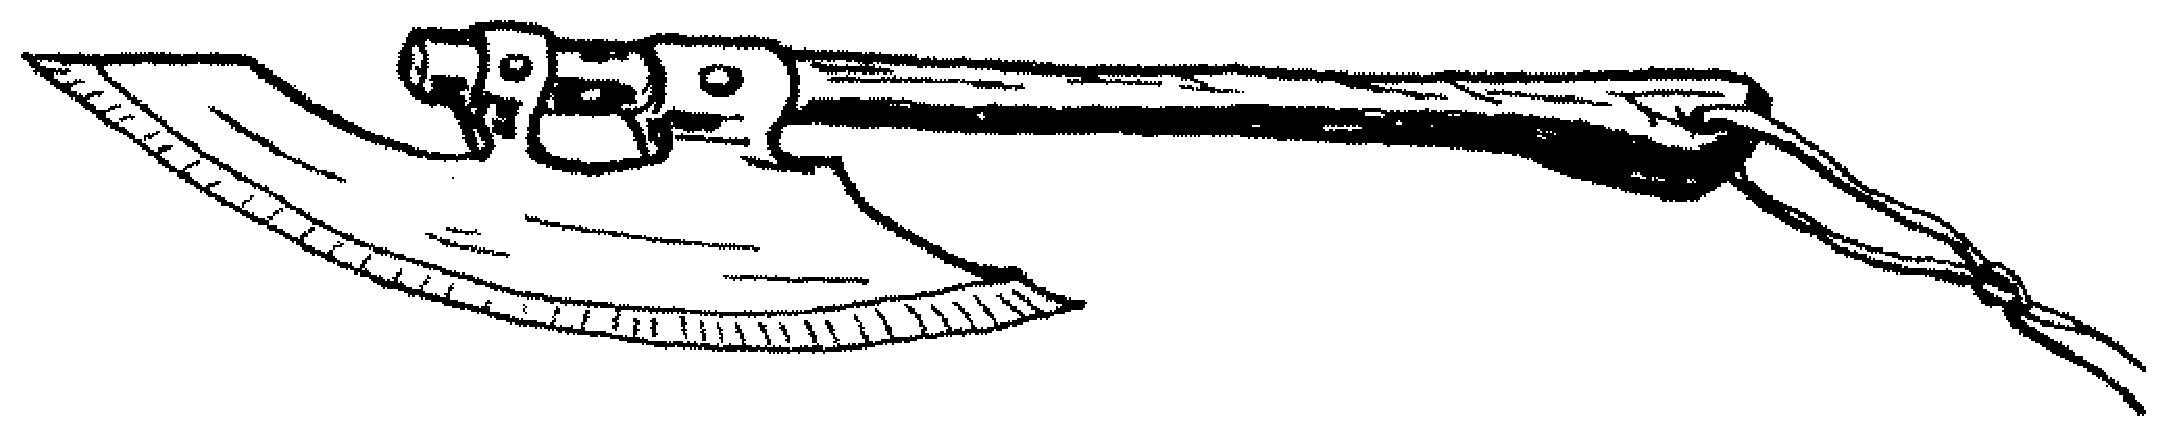
\epsfig{width=7.5cm,angle=0,file=/usr/local/share/midgard/axt1.ps}}
 \vspace*{2ex}
 \footnotesize
\parbox{7.7cm}
{
{\setlength{\tabcolsep}{1ex}\renewcommand{\arraystretch}{0.8}
    \begin{tabular}[b]{l|l|l|l|}
      \multicolumn{4}{l}{\small Grundkenntnisse in}\\\cline{2-2}\cline{4-4}
      ESchwert&\usebox{\ESchwert}&Kettenwaffe&\usebox{\Kettenwaffe}\\\cline{2-2}\cline{4-4}
      Stichwaffe&\usebox{\Stichwaffe}&Bogen&\usebox{\Bogen}\\\cline{2-2}\cline{4-4}
      ESchlagwaffe&\usebox{\ESchlagwaffe}&Armbrust&\usebox{\Armbrust}\\\cline{2-2}\cline{4-4}
      Spie�waffe&\usebox{\Spiesswaffe}&Schleuder&\usebox{\Schleuder}\\\cline{2-2}\cline{4-4}
      ZSchwert&\usebox{\ZSchwert}&Wurfspie�&\usebox{\Wurfspiess}\\\cline{2-2}\cline{4-4}
      ZSchlagwaffe&\usebox{\ZSchlagwaffe}&WSchlagwaffe&\usebox{\WSchlagwaffe}\\\cline{2-2}\cline{4-4}
      Stangenwaffe&\usebox{\Stangenwaffe}&Schild&\usebox{\Schilde}\\\cline{2-2}\cline{4-4}
    \end{tabular}}
\hfill
\LI
\scriptsize
{\setlength{\tabcolsep}{0.2ex}
    \begin{tabular}[b]{|c|c|}\hline
      R�stungs-&auf LP\\
      klasse&Verlust\\\hline
%      \rule{0ex}{0ex}&\\\hline
      \usebox{\ruestung}&\usebox{\ruestunglp}\\\hline
      \multicolumn{2}{c}{}\\\hline
      &mit Vert.\\
      \raisebox{1.5ex}[-1.5ex]{Abwehr}&Waffe\\\hline
       \rule{0ex}{0ex}\usebox{\abwehrfinal}&\\\hline
    \end{tabular}
}
}
\vspace{2ex}
{\renewcommand{\arraystretch}{0.7}
\begin{tabularx}{7.5cm}{lrXlr}
\multicolumn{5}{c}{\small Universelle Fertigkeiten}\\[1ex]
Balancieren&+8&&Schleichen&+1\\
Beredsamkeit&+3&&Schlittenfahren&+3\\
Beschatten&+3&&Schl�sser �ffnen&+0\\
Bet�uben&+6&&Schwimmen&+3\\
Fallen&+8&&Seilkunst&+4\\
Fallen entdecken&+0&&Springen&+8\\
Fallen entsch�rfen&+0&&Spurenlesen&+0\\
Fallenstellen&+1&&Stehlen&+3\\
Fangen&+8&&Tarnen&+1\\
Geheimmech. �ffnen&+1&&Tauchen&+9\\
Gel�ndelauf&+8&&�berleben&+6\\
Horchen&+2&&Verf�hren&+3\\
Kanufahren&+3&&Verh�ren&+3\\
Klettern&+8&&Verkleiden&+5\\
Landeskunde&+6&&Wagenlenken&+3\\
Meucheln&+0&&Wahrnehmung&+2\\
Reiten&+5&&Winden&+0\\
Rudern&+3&&&\\
\end{tabularx}}
\end{minipage}
%}
\end{document}


%%% Local Variables: 
%%% mode: latex
%%% TeX-master: t
%%% End: 
